% Options for packages loaded elsewhere
\PassOptionsToPackage{unicode}{hyperref}
\PassOptionsToPackage{hyphens}{url}
%
\documentclass[
  ignorenonframetext,
]{beamer}
\usepackage{pgfpages}
\setbeamertemplate{caption}[numbered]
\setbeamertemplate{caption label separator}{: }
\setbeamercolor{caption name}{fg=normal text.fg}
\beamertemplatenavigationsymbolsempty
% Prevent slide breaks in the middle of a paragraph
\widowpenalties 1 10000
\raggedbottom
\setbeamertemplate{part page}{
  \centering
  \begin{beamercolorbox}[sep=16pt,center]{part title}
    \usebeamerfont{part title}\insertpart\par
  \end{beamercolorbox}
}
\setbeamertemplate{section page}{
  \centering
  \begin{beamercolorbox}[sep=12pt,center]{part title}
    \usebeamerfont{section title}\insertsection\par
  \end{beamercolorbox}
}
\setbeamertemplate{subsection page}{
  \centering
  \begin{beamercolorbox}[sep=8pt,center]{part title}
    \usebeamerfont{subsection title}\insertsubsection\par
  \end{beamercolorbox}
}
\AtBeginPart{
  \frame{\partpage}
}
\AtBeginSection{
  \ifbibliography
  \else
    \frame{\sectionpage}
  \fi
}
\AtBeginSubsection{
  \frame{\subsectionpage}
}
\usepackage{amsmath,amssymb}
\usepackage{lmodern}
\usepackage{iftex}
\ifPDFTeX
  \usepackage[T1]{fontenc}
  \usepackage[utf8]{inputenc}
  \usepackage{textcomp} % provide euro and other symbols
\else % if luatex or xetex
  \usepackage{unicode-math}
  \defaultfontfeatures{Scale=MatchLowercase}
  \defaultfontfeatures[\rmfamily]{Ligatures=TeX,Scale=1}
\fi
\usetheme[]{Ilmenau}
\usecolortheme{beaver}
\usefonttheme{structurebold}
% Use upquote if available, for straight quotes in verbatim environments
\IfFileExists{upquote.sty}{\usepackage{upquote}}{}
\IfFileExists{microtype.sty}{% use microtype if available
  \usepackage[]{microtype}
  \UseMicrotypeSet[protrusion]{basicmath} % disable protrusion for tt fonts
}{}
\makeatletter
\@ifundefined{KOMAClassName}{% if non-KOMA class
  \IfFileExists{parskip.sty}{%
    \usepackage{parskip}
  }{% else
    \setlength{\parindent}{0pt}
    \setlength{\parskip}{6pt plus 2pt minus 1pt}}
}{% if KOMA class
  \KOMAoptions{parskip=half}}
\makeatother
\usepackage{xcolor}
\newif\ifbibliography
\usepackage{color}
\usepackage{fancyvrb}
\newcommand{\VerbBar}{|}
\newcommand{\VERB}{\Verb[commandchars=\\\{\}]}
\DefineVerbatimEnvironment{Highlighting}{Verbatim}{commandchars=\\\{\}}
% Add ',fontsize=\small' for more characters per line
\usepackage{framed}
\definecolor{shadecolor}{RGB}{248,248,248}
\newenvironment{Shaded}{\begin{snugshade}}{\end{snugshade}}
\newcommand{\AlertTok}[1]{\textcolor[rgb]{0.94,0.16,0.16}{#1}}
\newcommand{\AnnotationTok}[1]{\textcolor[rgb]{0.56,0.35,0.01}{\textbf{\textit{#1}}}}
\newcommand{\AttributeTok}[1]{\textcolor[rgb]{0.77,0.63,0.00}{#1}}
\newcommand{\BaseNTok}[1]{\textcolor[rgb]{0.00,0.00,0.81}{#1}}
\newcommand{\BuiltInTok}[1]{#1}
\newcommand{\CharTok}[1]{\textcolor[rgb]{0.31,0.60,0.02}{#1}}
\newcommand{\CommentTok}[1]{\textcolor[rgb]{0.56,0.35,0.01}{\textit{#1}}}
\newcommand{\CommentVarTok}[1]{\textcolor[rgb]{0.56,0.35,0.01}{\textbf{\textit{#1}}}}
\newcommand{\ConstantTok}[1]{\textcolor[rgb]{0.00,0.00,0.00}{#1}}
\newcommand{\ControlFlowTok}[1]{\textcolor[rgb]{0.13,0.29,0.53}{\textbf{#1}}}
\newcommand{\DataTypeTok}[1]{\textcolor[rgb]{0.13,0.29,0.53}{#1}}
\newcommand{\DecValTok}[1]{\textcolor[rgb]{0.00,0.00,0.81}{#1}}
\newcommand{\DocumentationTok}[1]{\textcolor[rgb]{0.56,0.35,0.01}{\textbf{\textit{#1}}}}
\newcommand{\ErrorTok}[1]{\textcolor[rgb]{0.64,0.00,0.00}{\textbf{#1}}}
\newcommand{\ExtensionTok}[1]{#1}
\newcommand{\FloatTok}[1]{\textcolor[rgb]{0.00,0.00,0.81}{#1}}
\newcommand{\FunctionTok}[1]{\textcolor[rgb]{0.00,0.00,0.00}{#1}}
\newcommand{\ImportTok}[1]{#1}
\newcommand{\InformationTok}[1]{\textcolor[rgb]{0.56,0.35,0.01}{\textbf{\textit{#1}}}}
\newcommand{\KeywordTok}[1]{\textcolor[rgb]{0.13,0.29,0.53}{\textbf{#1}}}
\newcommand{\NormalTok}[1]{#1}
\newcommand{\OperatorTok}[1]{\textcolor[rgb]{0.81,0.36,0.00}{\textbf{#1}}}
\newcommand{\OtherTok}[1]{\textcolor[rgb]{0.56,0.35,0.01}{#1}}
\newcommand{\PreprocessorTok}[1]{\textcolor[rgb]{0.56,0.35,0.01}{\textit{#1}}}
\newcommand{\RegionMarkerTok}[1]{#1}
\newcommand{\SpecialCharTok}[1]{\textcolor[rgb]{0.00,0.00,0.00}{#1}}
\newcommand{\SpecialStringTok}[1]{\textcolor[rgb]{0.31,0.60,0.02}{#1}}
\newcommand{\StringTok}[1]{\textcolor[rgb]{0.31,0.60,0.02}{#1}}
\newcommand{\VariableTok}[1]{\textcolor[rgb]{0.00,0.00,0.00}{#1}}
\newcommand{\VerbatimStringTok}[1]{\textcolor[rgb]{0.31,0.60,0.02}{#1}}
\newcommand{\WarningTok}[1]{\textcolor[rgb]{0.56,0.35,0.01}{\textbf{\textit{#1}}}}
\usepackage{longtable,booktabs,array}
\usepackage{calc} % for calculating minipage widths
\usepackage{caption}
% Make caption package work with longtable
\makeatletter
\def\fnum@table{\tablename~\thetable}
\makeatother
\usepackage{graphicx}
\makeatletter
\def\maxwidth{\ifdim\Gin@nat@width>\linewidth\linewidth\else\Gin@nat@width\fi}
\def\maxheight{\ifdim\Gin@nat@height>\textheight\textheight\else\Gin@nat@height\fi}
\makeatother
% Scale images if necessary, so that they will not overflow the page
% margins by default, and it is still possible to overwrite the defaults
% using explicit options in \includegraphics[width, height, ...]{}
\setkeys{Gin}{width=\maxwidth,height=\maxheight,keepaspectratio}
% Set default figure placement to htbp
\makeatletter
\def\fps@figure{htbp}
\makeatother
\setlength{\emergencystretch}{3em} % prevent overfull lines
\providecommand{\tightlist}{%
  \setlength{\itemsep}{0pt}\setlength{\parskip}{0pt}}
\setcounter{secnumdepth}{-\maxdimen} % remove section numbering
\ifLuaTeX
  \usepackage{selnolig}  % disable illegal ligatures
\fi
\IfFileExists{bookmark.sty}{\usepackage{bookmark}}{\usepackage{hyperref}}
\IfFileExists{xurl.sty}{\usepackage{xurl}}{} % add URL line breaks if available
\urlstyle{same} % disable monospaced font for URLs
\hypersetup{
  pdftitle={Séance 4.2: Mesures de tendance centrale},
  pdfauthor={Visseho Adjiwanou, PhD.},
  hidelinks,
  pdfcreator={LaTeX via pandoc}}

\title{Séance 4.2: Mesures de tendance centrale}
\subtitle{Discussion en classe}
\author{Visseho Adjiwanou, PhD.}
\date{29 January 2023}

\begin{document}
\frame{\titlepage}

\begin{frame}{A quoi ça sert?}
\protect\hypertarget{a-quoi-uxe7a-sert}{}
\begin{itemize}
\tightlist
\item
  Une mesure de tendance centrale est une valeur \textbf{typique} ou
  \textbf{représentative} d'un ensemble de scores
\end{itemize}
\end{frame}

\begin{frame}{Résumé : Mesure de tendance centrale (paramètres de
position)}
\protect\hypertarget{ruxe9sumuxe9-mesure-de-tendance-centrale-paramuxe8tres-de-position}{}
\begin{longtable}[]{@{}lll@{}}
\toprule()
Symbole & Définition & Formules \\
\midrule()
\endhead
Moyenne & Somme des valeurs divisée par &
\(\bar{X} = \frac{1}{n} \sum_{i=1}^n X_i\) \\
& l'effectif de la série & \\
Médiane & Valeur qui divise la distribution & \\
& en deux parties égales & \\
Mode & Valeur observée de fréquence maximum & \\
Percentile & Valeurs qui divisent la distribution & \\
& en 100 parties égales & \\
\bottomrule()
\end{longtable}
\end{frame}

\begin{frame}{Résumé : Mesure de dispersion}
\protect\hypertarget{ruxe9sumuxe9-mesure-de-dispersion}{}
\begin{longtable}[]{@{}lll@{}}
\toprule()
Symbole & Définition & Formules \\
\midrule()
\endhead
Étendue & Différence entre la plus grande & G - P \\
& et la plus petite valeur de la & \\
& variable & \\
EIQ & 3ème quartile - 1er quartile & Q3 - Q1 \\
Déviation & La distance d'une valeur à & \(X - \bar{X}\) \\
& la moyenne & \\
Sommes & Somme des carrés des déviations & SC =
\(\sum_{i=1}^n(X_i-\bar{X})^2\) \\
des carrés & & \\
Variance & Moyenne des carrés des déviances &
\(s^2=\frac{1}{n-1}\sum_{i=1}^n(X_i-\bar{X})^2\) \\
Écart-type & Racine carrée de la variance &
\(s = \sqrt{\frac{1}{n-1} \sum_{i=1}^n(X_i-\bar{X})^2}\) \\
\bottomrule()
\end{longtable}
\end{frame}

\begin{frame}{Résumé : Quel type de résumé pour quel type de variable?}
\protect\hypertarget{ruxe9sumuxe9-quel-type-de-ruxe9sumuxe9-pour-quel-type-de-variable}{}
\begin{longtable}[]{@{}llll@{}}
\toprule()
Type de variable & Fréquence & Pourcentage & Commentaire \\
\midrule()
\endhead
Nominale & Oui & Oui & Toujours \\
Ordinale & Oui & Oui & Toujours \\
Ratio/Intervalle & Pas souhaité & Pas souhaité & Oui si peu de
modalités \\
Ratio/Intervalle & Oui & Oui & Toujours \\
(données groupées) & & & \\
\bottomrule()
\end{longtable}
\end{frame}

\begin{frame}{Résumé : Quel type de résumé pour quel type de variable?}
\protect\hypertarget{ruxe9sumuxe9-quel-type-de-ruxe9sumuxe9-pour-quel-type-de-variable-1}{}
\begin{longtable}[]{@{}llllll@{}}
\toprule()
Type de variable & Moyenne & Mode & Médiane & Variance & Écart-type \\
\midrule()
\endhead
Nominale & Non & Oui & Non & Non & Non \\
Ordinale & Possible & Oui & Oui & Possible & Possible \\
Ratio/Intervalle & Oui & Oui & Oui & Oui & Oui \\
Ratio/Intervalle & Oui & Oui & Oui & Oui & Oui \\
(données groupées) & & & & & \\
\bottomrule()
\end{longtable}
\end{frame}

\hypertarget{exemple-de-calcul}{%
\section{Exemple de calcul}\label{exemple-de-calcul}}

\begin{frame}{Distribution de revenu}
\protect\hypertarget{distribution-de-revenu}{}
Voici les revenus (en millier) d'un échantillon de 15 hommes et de 16
femmes

\begin{longtable}[]{@{}llllllll@{}}
\toprule()
ind & Revenus & ind & Revenus & ind & Revenus & ind & Revenus \\
\midrule()
\endhead
1 & 2 & 9 & 3.1 & 1 & 3.1 & 9 & 0.5 \\
2 & 2.5 & 10 & 1.4 & 2 & 2.7 & 10 & 1.3 \\
3 & 1.7 & 11 & 7.1 & 3 & 1.2 & 11 & 2.9 \\
4 & 3 & 12 & 6.0 & 4 & 4.2 & 12 & 2.7 \\
5 & 5 & 13 & 3.3 & 5 & 5.5 & 13 & 5.1 \\
6 & 4.1 & 14 & 4.3 & 6 & 4.3 & 14 & 3.0 \\
7 & 8.1 & 15 & 6.1 & 7 & 2.0 & 15 & 6.3 \\
8 & 5.2 & & & 8 & 1.5 & 16 & 4.2 \\
\bottomrule()
\end{longtable}
\end{frame}

\begin{frame}{Distribution du revenu des hommes}
\protect\hypertarget{distribution-du-revenu-des-hommes}{}
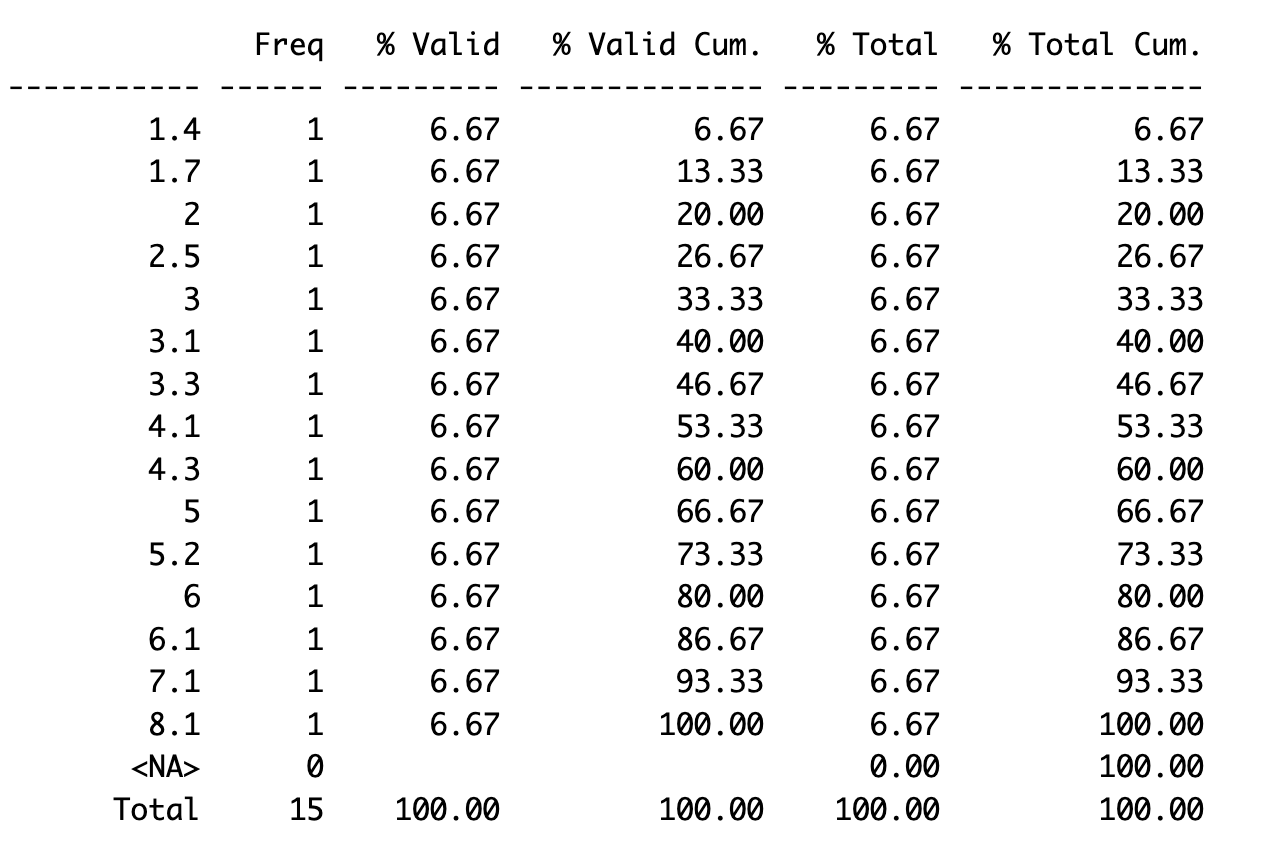
\includegraphics{../../Images/cours4.1.png}
\end{frame}

\begin{frame}[fragile]{Moyenne}
\protect\hypertarget{moyenne}{}
\begin{verbatim}
- Revenu moyen des hommes = (2 + 2.5 + 1.7 + 3 + 5 + 4.1 + 8.1 + 5.2 + 3.1 + 1.4 + 7.1 + 6.0 + 3.3 + 4.3 + 6.1) / 15

- revenu moyen des hommes = 4.19

- Revenu moyen des femmes = (3.1 + 2.7 + 1.2 + 4.2 + 5.5 + 4.3 + 2.0 + 1.5 + 0.5 + 1.3 + 2.9 + 2.7 + 5.1 + 3.0 + 6.3 + 4.2)/16
- Revenu moyen des femmes = 3.16
\end{verbatim}
\end{frame}

\begin{frame}{Médiane des hommes}
\protect\hypertarget{muxe9diane-des-hommes}{}
Médiane: valeur qui partage la distribution en deux parties égales

\begin{itemize}
\item
  \textbf{La Médiane} = valeur telle que la moitié des observations lui
  sont inférieures et donc la moitié lui sont supérieures.
\item
  C'est donc assez facile à calculer, il suffit juste d'ordonner les
  cas.
\item
  Milieu de la distribution = (15 + 1)/2 = 8
\end{itemize}

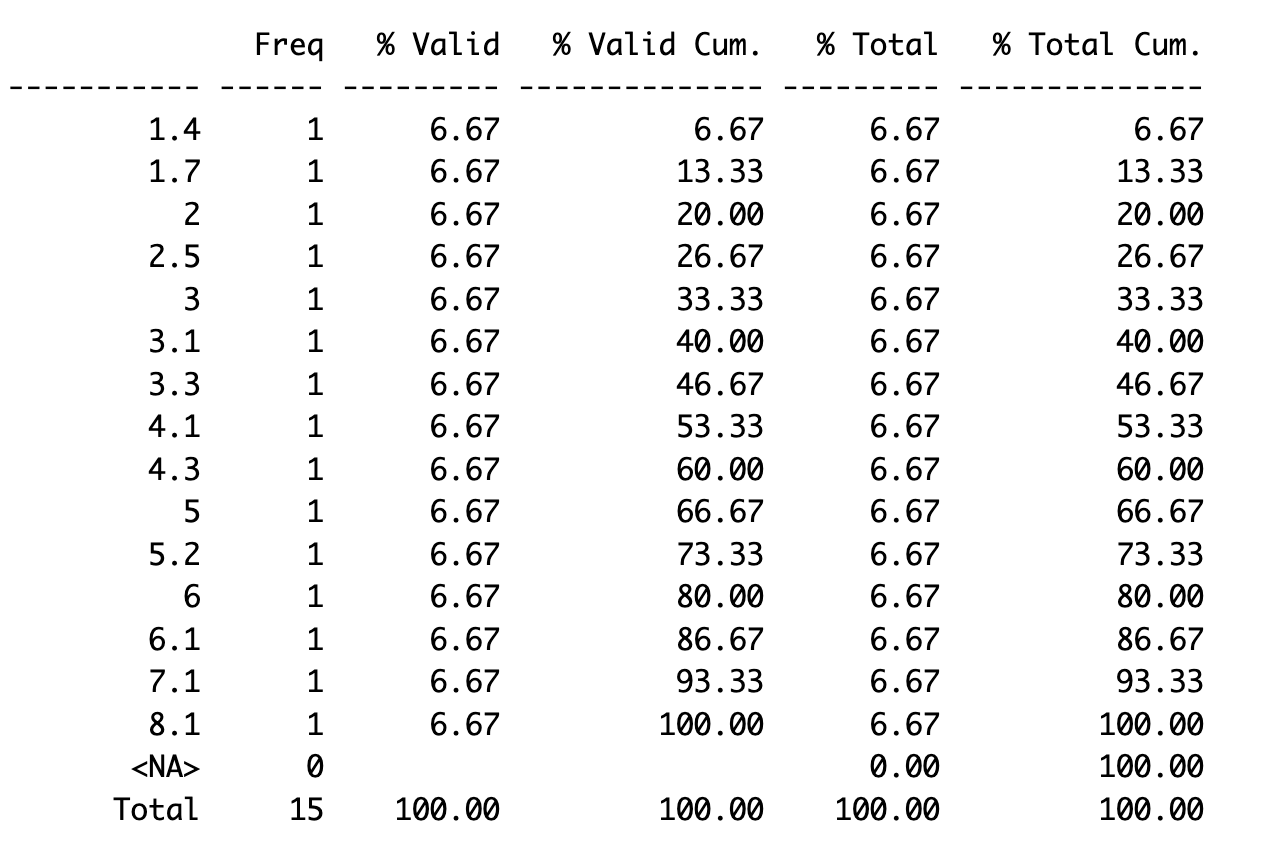
\includegraphics{../../Images/cours4.1.png} 25\% des gens ont un revenu
inférieur à cette valeur

\begin{itemize}
\item
  je vois que 20\% des gens ont un revenu de 2 ou moins
\item
  26,67\% des gens ont in revenu de 2.5 ou moins donc le 1e quartile se
  trouve entre 2 et 2.5
\item
  Médiane Homme = 4.1
\end{itemize}
\end{frame}

\begin{frame}{Médiane des femmes}
\protect\hypertarget{muxe9diane-des-femmes}{}
Milieu de la distribution : (16 +1)/2 = 8.5 entre la 8 et la 9e valeur

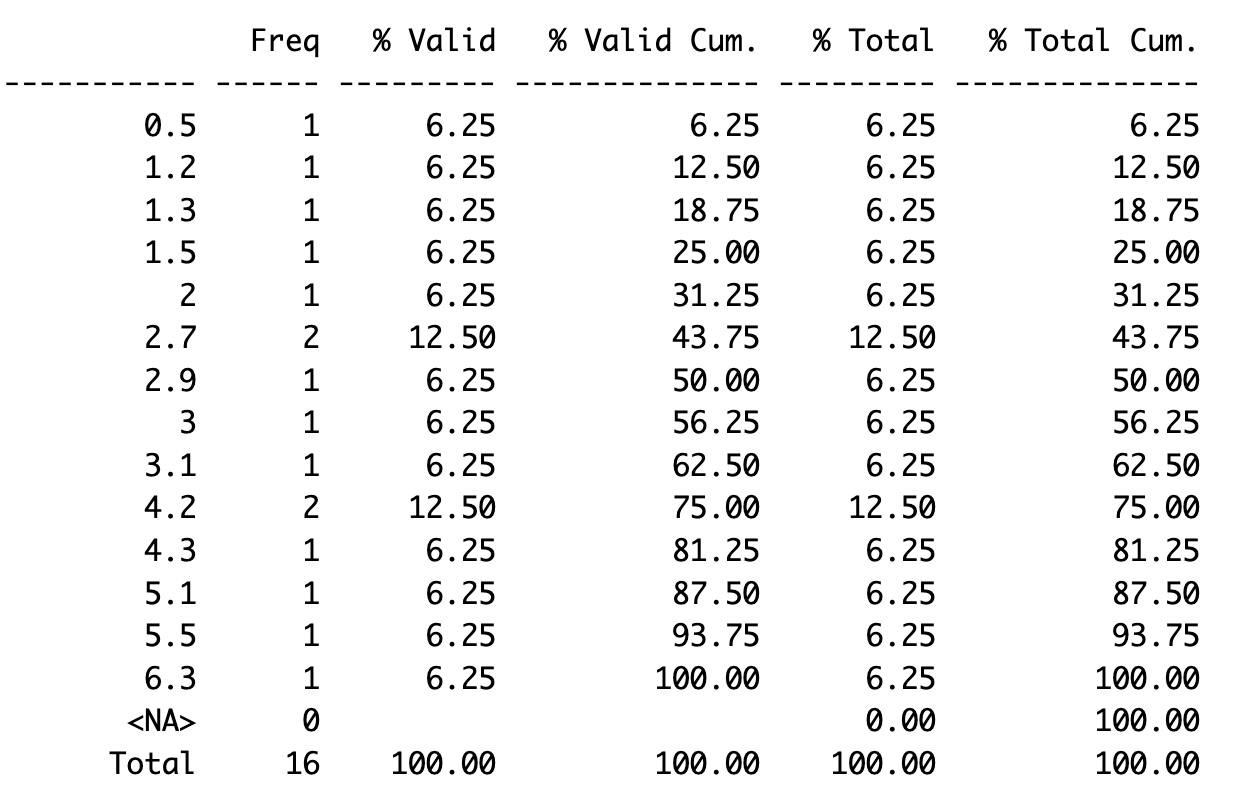
\includegraphics{../../Images/cours4.2.jpg} Médiane se situe entre la 8e
et la 9e valeur

Médiane = (2.9 + 3)/2 = 2.95
\end{frame}

\begin{frame}{Mode}
\protect\hypertarget{mode}{}
\begin{itemize}
\tightlist
\item
  Homme = il n'y a pas de mode
\item
  Femme = deux modes, 2.7 et 4.2
\end{itemize}
\end{frame}

\begin{frame}{Premier quartile}
\protect\hypertarget{premier-quartile}{}
Quelle est la localisation du premier quartile?

1 2 3 4 5 6 7 8 9 10 11 12 13 17 15\\
1.4 1.7 2 2.5 3 3.1 3.3 4.1 4.3 5 5.2 6 6.1 7.1 8.1
\end{frame}

\begin{frame}{Premier quartile}
\protect\hypertarget{premier-quartile-1}{}
Quelle est la localisation du premier quartile?

\(L_k = k/100*(n + 1)\)

k = 25 si premier quartile n = 15

donc l\_25 = 25/100*(15+1) = 4 Le premier quartile se trouve donc à la
4e position

premier quartile (Q1) = 2.5
\end{frame}

\begin{frame}{Troisième quartile}
\protect\hypertarget{troisiuxe8me-quartile}{}
l\_75 = 75/100*(15+1) = 12

donc Q3 = 6
\end{frame}

\begin{frame}{Et pour les femmes?}
\protect\hypertarget{et-pour-les-femmes}{}
Q1 = ? Q3 = ?
\end{frame}

\begin{frame}{Et pour les femmes}
\protect\hypertarget{et-pour-les-femmes-1}{}
1 2 3 4 \textbar{} 5 6 7 8 \textbar{} 9 10 11 12 \textbar{} 13 14 15 16
.5 1.2 1.3 1.5 \textbar{} 2 2.7 2.7 2.9 \textbar{} 3. 3.1 4.2 4.2
\textbar{} 4.3 5.1 5.5 6.3
\end{frame}

\begin{frame}{Et pour les femmes?}
\protect\hypertarget{et-pour-les-femmes-2}{}
L\_25 = 25/100\emph{(16+1) = 4.25 (entre 4 et 5) L\_75 = 75/100}(16+1) =
12.75 (entre 12 et 13)

Q1 = (1.5 + 2)/2 = 1.75 Q3 = (4.2 + 4.3)/2 = 4.25

\begin{itemize}
\tightlist
\item
  Une difficulté arrive avec les variables ordinales
\end{itemize}
\end{frame}

\begin{frame}{Représentation}
\protect\hypertarget{repruxe9sentation}{}
\begin{itemize}
\tightlist
\item
  Boxplot
\end{itemize}

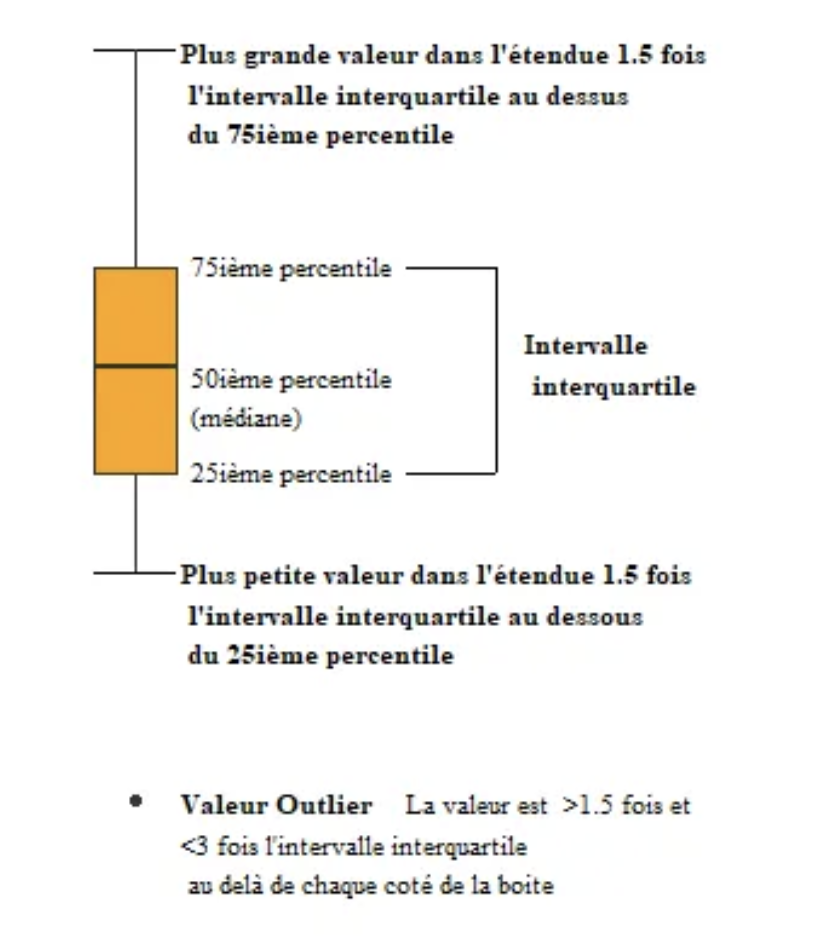
\includegraphics{../../Images/boxplot_interpretation.png}
\end{frame}

\begin{frame}{Représentation}
\protect\hypertarget{repruxe9sentation-1}{}
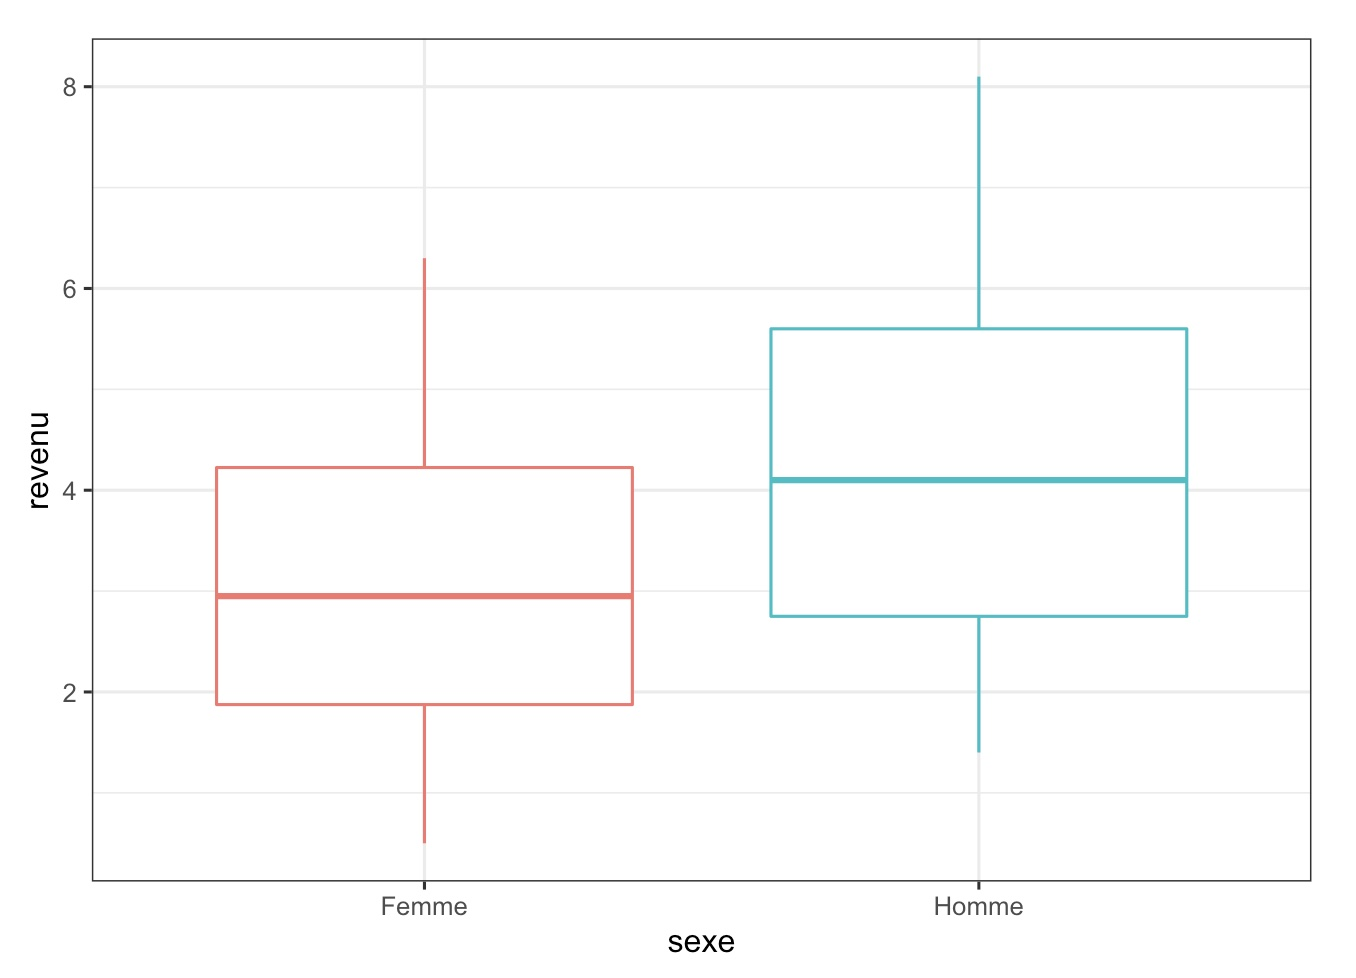
\includegraphics{../../Images/cours4_graph1.jpg}
\end{frame}

\begin{frame}{Médiane des variables ordinales}
\protect\hypertarget{muxe9diane-des-variables-ordinales}{}
Exemple: Attitude envers les immigrants et les emplois

\begin{itemize}
\tightlist
\item
  Q1: Sur une échelle de 1 (totalement en désaccord) à 5 (totalement
  d'accord), que pensez-vous de l'affirmation suivante: ``Les immigrants
  volent nos emplois''
\end{itemize}
\end{frame}

\begin{frame}{Médiane des variables ordinales}
\protect\hypertarget{muxe9diane-des-variables-ordinales-1}{}
\begin{longtable}[]{@{}llllc@{}}
\toprule()
Valeur & Fréquence & Fréq. cumulée & Pourcentage & Pourc. cumulé \\
\midrule()
\endhead
1 & 170 & 170 & & \\
2 & 446 & 616 & & \\
3 & 299 & 915 & & \\
4 & 301 & 1216 & & \\
5 & 65 & 1281 & & \\
N & 1281 & & & \\
\bottomrule()
\end{longtable}

\begin{itemize}
\tightlist
\item
  Médiane va diviser la distribution en deux partie égale
\item
  (1281 + 1)/2 = 641
\item
  la médiane est la valeur du 641e score, c'est-à-dire quelque part
  parmi les 299 scores 3
\item
  La médiane est donc 3. Cependant il faut affiner cela.
\end{itemize}
\end{frame}

\begin{frame}{Médiane des variables ordinales}
\protect\hypertarget{muxe9diane-des-variables-ordinales-2}{}
\begin{itemize}
\tightlist
\item
  Convention: on va supposer que derrière les réponses à cette question,
  il y a une échelle (ratio) allant de 0.5 à 5.5.
\item
  Autrement dit, ceux qui ont répondu 1, aurait répondu en réalité entre
  0.5 et 1.5. On les ramène donc à la moyenne de l'intervalle qui vaut
  (0.5 + 1.5)/2 = 1
\item
  Ainsi, les 299 personnes qui ont répondu 3 ont en fait répondu entre
  2.5 et 3.5
\item
  Nous allons donc interpoler pour trouver à quel endroit se situe la
  médiane
\end{itemize}

617 ---------641-------------------------------------617+299 = 916

2.5 ----------M--------------------------------------3.5
\end{frame}

\begin{frame}{Médiane des variables ordinales}
\protect\hypertarget{muxe9diane-des-variables-ordinales-3}{}
\begin{itemize}
\tightlist
\item
  Interpolation
\item
  Application de la règle de trois
\item
  Si 3 pains coûtent 55\$, combien coûte 2 pains?
\end{itemize}

(M - 3.5)/(2.5 - 3.5) = (641 - 916)/(617 - 916)

M = {[}(641 - 916)/(617 - 916){]}/(2.5 - 3.5) + 3.5

M = 2.6
\end{frame}

\begin{frame}{Vous pouvez préféré utiliser la formule du livre}
\protect\hypertarget{vous-pouvez-pruxe9fuxe9ruxe9-utiliser-la-formule-du-livre}{}
\[Md = L + (\frac{N/2 - F}{f})(i)\] - L = la limite inférieure de
l'intervalle contenant la médiane (2.5) - N = le nombre de cas (1281) -
F = la fréquence cumulative des scores inférieurs à l'intervalle
contenant la médiane (616) - f = le nombre de scores que comprend
l'intervalle contenant la médiane (299) - i = la largeur de l'intervalle
contenant la médiane (1)

Md = 2.5 +(1281/2 - 616)/299*1 = 2.6
\end{frame}

\hypertarget{exemple-dapplication}{%
\section{Exemple d'application}\label{exemple-dapplication}}

\begin{frame}[fragile]{Pour la semaine prochaine}
\protect\hypertarget{pour-la-semaine-prochaine}{}
\begin{enumerate}
\tightlist
\item
  Lecture
\end{enumerate}

\begin{itemize}
\tightlist
\item
  Paramètres de variation (ou de dispersion) - Fox : chapitre 4,
  pp.91-103
\item
  Distribution d'échantillonnage - Fox : Chapitre 4, pp.103-120
\end{itemize}

\begin{enumerate}
\setcounter{enumi}{1}
\tightlist
\item
  Application
\end{enumerate}

\begin{itemize}
\tightlist
\item
  \url{https://juba.github.io/tidyverse/01-presentation.html}
\item
  \url{https://juba.github.io/tidyverse/02-prise_en_main.html}
\item
  \url{https://juba.github.io/tidyverse/03-premier_travail.html}
\end{itemize}

\begin{Shaded}
\begin{Highlighting}[]
\FunctionTok{ggplot}\NormalTok{(donnee\_revenu) }\SpecialCharTok{+}
  \FunctionTok{geom\_boxplot}\NormalTok{(}\FunctionTok{aes}\NormalTok{(}\AttributeTok{x =}\NormalTok{ sexe, }\AttributeTok{y =}\NormalTok{ revenu, }\AttributeTok{color =}\NormalTok{ sexe)) }\SpecialCharTok{+}
  \FunctionTok{theme\_bw}\NormalTok{()}
\end{Highlighting}
\end{Shaded}

\includegraphics{Seance4.2_Mesures_tendances_centrales_cours_files/figure-beamer/unnamed-chunk-1-2.pdf}

--\textgreater{}
\end{frame}

\end{document}
